
\chapter{Estudo dos Dados}
\label{cap:estudodados}


\section{Limpeza dos Dados}

\subsection{Contagem de dias válidos}

Para treinar algum tipo de modelo preditivo com os dados, é necessário parear dados de entrada e de saída. Para os diversos conjuntos de dados cedidos pela Intercement, os mesmos representam diferentes momentos da produção de cimento. Então ao usarmos algum desses dados como entrada para prever uma saída, devemos adicionar o delay temporal correspondente ao tempo que demora para entrada se tornar saída. Por exemplo, se tentarmos prever os dados de expedição com os dados de farinha, o delay apropriado é de 10 dias. No restante desse documento esse delay sempre foi considerado independente de quais dados estejam sendo usados.

Também devemos notar o fato que a frequência na qual os dados de Clínquer, Farinha e Cimento Cru são anotados é bastante maior que a frequência temporal dos dados de expedição. O que também dificulta o pareamento. Por exemplo, temos dados de Clínquer a cada hora, sendo que os dados de expedição são anotados dia a dia. Portanto, foi necessário unir dados de um mesmo dia (tirando a média das suas entradas) para que fosse possível associar diferentes conjuntos de dados de um para um.
\begin{enumerate}
    \item Os dados de  Clínquer possuem 3528 linhas de dados de 2936 dias distintos
\item Os dados de  Expedição possuem 3650 linhas de dados de 2520 dias distintos
\item Os dados de  Farinha possuem 3530 linhas de dados de 2937 dias distintos
\item Os dados de  Cru possuem 30558 linhas de dados de 30558 dias distintos
\end{enumerate}

\subsection{Dados faltantes}
Embora tenhamos uma quantidade razoável de dias com dados presentes, esses muitas vezes não possuem alguma de suas colunas.
A seguir vemos para todos os dataframes, para cada uma de suas colunas, quantos dias possuem dados faltantes.



\captionof{table}{Dias com dados faltantes para cada parâmetro de Clínquer}
\begin{center}
\begin{tabular}{ c c }
 CaOL       &      596\\
Fe2O3       &    596\\
CaO         &   596\\
SiO2        &  596\\
Al2O3       & 596\\
P2O5        & 596\\
MgO         & 596\\
K2O         & 596\\
Na2O        & 596\\
CLOR        & 2724\\
FLUOR       & 2095\\
MS          & 596\\
MA          & 596\\
FSC         & 596\\
RSA         & 809\\
C3S         & 596\\
C2S         & 596\\
C3A         & 596\\
C4AF        & 596\\
F.liq       & 596\\
25,4 mm     & 2753\\
12,7 mm     & 2752\\
6,35  mm    & 2752\\
3,36 mm     & 2752\\
\textless 3,36 mm    & 2756
\end{tabular}
\end{center}
\newpage
\captionof{table}{Dias com dados faltantes para cada parâmetro de Expedição}
\begin{center}
\begin{tabular}{ c c }
AGP     &  1131\\
IP      &  1131\\
FP      &  1132\\
G75    &  1133\\
G44   &  1153\\
MVOL    &  1656\\
SBL     &  1131\\
RC3     &  1130\\
RC7     &  1130\\
RC28    &  1130\\
RICARB  &  1331\\
PF      &  1136\\
AL2O3   &  1140\\
CAOT    &  1140\\
K2O     &  1140\\
MGO     &  1139\\
SIO2    &  1140\\
FE2O3   &  1140\\
SO3     &  1137\\
NA2O    &  3139\\
P2O5    &  1141\\
EXP     &  2804\\
RC1     &  1861\\
RC91    &  3638\\
CO2     &  3629 
\end{tabular}
\end{center}

\newpage

\captionof{table}{Dias com dados faltantes para cada parâmetro de Farinha}
\begin{center}
\begin{tabular}{ c c }
Fe2O3     &   595\\
CaO       &  595\\
SiO2      &   595\\
Al2O3     &   595\\
SO3       &   595\\
P2O5      &   595\\
MgO       &   595\\
K2O       &   595\\
Na2O      &   931\\
CLOR.     &  1697\\
FLUOR.    &  1588\\
FSC       &   595\\
MS        &   595\\
MA        &   595\\
RSA       &   815\\
P. F AL.  &   593 \\
\end{tabular}
\end{center}

\newpage

\captionof{table}{Dias com dados faltantes para cada parâmetro de Cimento Cru}
\begin{center}
\begin{tabular}{ c c }
Alim. (t/h)       & 131\\
Prod (ton)        & 250\\
Calc. (\%)        & 131\\
Arg. (\%)         & 131\\
Areia (\%)        & 132\\
Corr. (\%)        & 370\\
Caulim (\%)       & 421\\
Cinza (\%)        & 295\\
Alurox (\%)       & 442\\
Fe2O3             & 44\\
CaO               & 44\\
SiO2              & 44\\
Al2O3             & 44\\
SO3               & 44\\
P2O5              & 44\\
MgO              &  44\\
K2O              &  44\\
Na2O             &  48\\
MA               &  44\\
MS               &  44\\
FSC              &  44\\
\#100             & 187\\
\#170             &  44\\
Umid Calc (\%)   &  413\\
Umid Arg (\%)    &  414 \\
Umid Areia (\%) &    391 \\
\end{tabular}
\end{center}




\subsection{Resample dos dados}
Para maior facilidade de manuseio dos dados. Foi necessário realizar um \textbf{resample}. Os dados foram modificados para que entradas realizadas no mesmo dia sejam unificadas. E dias sem dados foram criados como placeholders para facilidade de vizualiação dos dados. A seguir são reproduzidas as contagens de dados após o resample.


\begin{itemize}
\item Clínquer: Temos dados de entrada do dia 22/04/2008 até o dia 18/12/2017
\item Clínquer: De um período de 3528 dias temos 2932 dias preenchidos com dados de entrada
\item Expedição: Temos dados de entrada do dia 02/01/2008 até o dia 29/12/2017
\item Expedição: De um período de 3650 dias temos 2520 dias preenchidos com dados de entrada
\item Farinha: Temos dados de entrada do dia 20/04/2008 até o dia 18/12/2017
\item Farinha: De um período de 3530 dias temos 2937 dias preenchidos com dados de entrada
\item Cru: Temos dados de entrada do dia 21/04/2008 até o dia 09/12/2016
\item Cru: De um período de 3155 dias temos 2675 dias preenchidos com dados de entrada
\end{itemize}


\section{Testes de Sazonalidade}

Diversas publicações recentes estudam a eficácia de modelos de Deep Learning para predição de séries temporais, como consumo de energia elétrica. Os dados estudados nesse documento são séries temporais dado que são indexados pelo tempo, porém, resta analisar características temporais desses dados. No exemplo do consumo de energia elétrica, poderiamos notar que, ao longo de vários anos presentes nos dados, o consumo de energia de uma certa residência aumenta em determinado mês. Isso seria um fator útil que um modelo poderia aprender para a predição futura do consumo dessa residência. Dados que não possuem nenhuma característica temporal (i.e. a ordem não importa) seriam por exemplo provenientes de um estudo do salário recebido por uma amostra da população dados fatores como gênero, escolaridade e idade. No primeiro exemplo temos um caso de \textbf{sazonalidade} nos dados, algo que pode ser analisado em séries temporais com testes de análise espectral e auto-correlação. Para os dados desse problema, iremos testar a sazonalidade dos preditores de dureza do cimento.

\subsection{Análise Espectral}

Uma maneira de testar sazonalidade de dados indexados temporalmente é usar a técnica de Transformada de Fourier, onde podemos estudar quais frequencias dentro de um espectro podem ser usadas para decompor um sinal (i.e. nossos dados). Para essa análise usamos os índices de dureza contidos nos dados de expedição, de 2008 até 2014 e descartamos a parte imaginária da análise já que nossos dados não possuem parte complexa. Seguem os resultados:


\begin{figure}[H]
\centering
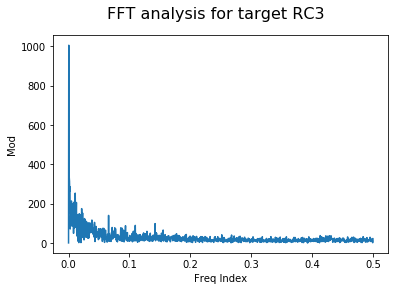
\includegraphics[width=0.9\columnwidth]{FFT_RC3.png}
\caption{Análise Espectral para preditor RC3}
\end{figure}

\begin{figure}[H]
\centering
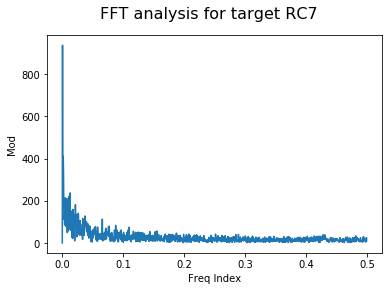
\includegraphics[width=0.9\columnwidth]{FFT_RC7.png}
\caption{Análise Espectral para preditor RC7}
\end{figure}

\begin{figure}[H]
\centering
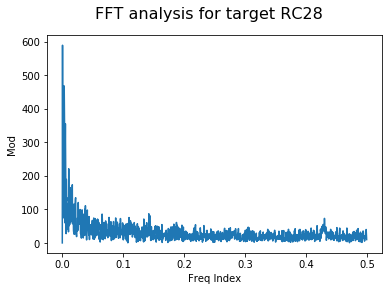
\includegraphics[width=0.9\columnwidth]{FFT_RC28.png}
\caption{Análise Espectral para preditor RC28}
\end{figure}


Podemos notar que a "energia" do sinal não possui picos em nenhuma frequência além da frequência zero, que seria a potência média do sinal, ou seja, uma componente que não depende do tempo. Então, afirmamos que esses dados não possuem sazonalidade mensal ou anual. O que significa que a média e a variância desses indicadores não possuem trends e.g. alguma mudança similar todo mês de Janeiro.


